\documentclass{jhwhw}
	\usepackage{enumitem}
	\usepackage{soul}
	\usepackage{float}
	
	\title{EE 4341 Homework 2}
    \author{Alex Biedny}
    \date{\today}
    \chead{EE 4341 Homework 2}
    \lhead{Alex Biedny}
    
\usepackage{graphicx}
\begin{document}

\maketitle

\problem{}
\begin{enumerate}
\item It is reentrant. There are no global or static variables used that could be modified elsewhere during an interrupt, and the function state can't be changed outside of itself.
\item
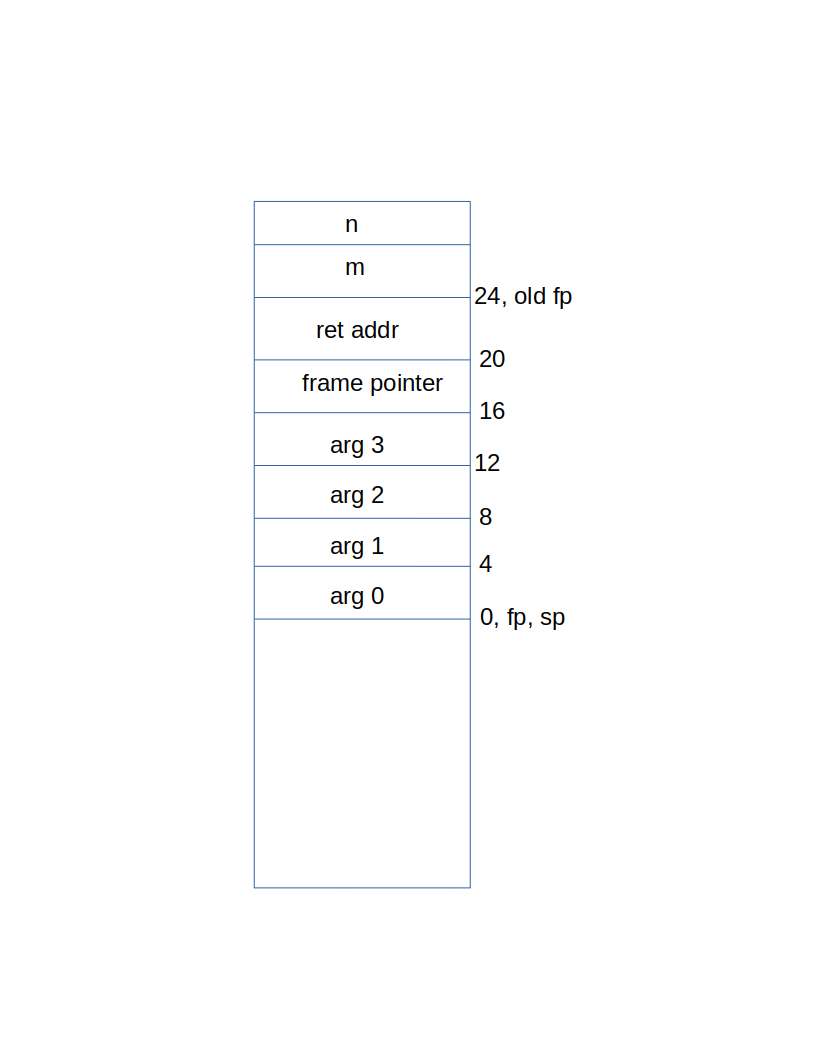
\includegraphics[scale=0.50]{HW2-1.png}
\item Each function frame needs 24 bytes on that stack, and the function will be recursively called three times, meaning that the stack needs 72 bytes to compute the GCD. The value returned will be 6.
\end{enumerate}

\problem{}
\begin{enumerate}
\item \begin{verbatim}
void __ISR(_TIMER_1_VECTOR,IPL4SOFT) Timer1ISR(void) {
    if (counter == 0) {
        ISRdevice0();
    }
    else if (counter == 1) {
        ISRdevice1();
    }
    else if (counter == 2) {
        ISRdevice2();
    }
    counter = (++counter) % 3;
}
\end{verbatim}
\item \begin{verbatim}
T1CON = 0x0;
TMR1 = 0x0;
PR1 = 0xFFFF;
    
IPC1SET = 0x0001;
    
T1CONbits.ON = 1;
\end{verbatim}
\end{enumerate}

\problem{}
\begin{enumerate}
\item \begin{verbatim}
uint16_t Buffer[64];
uint16_t *Front = &Buffer[0];
uint16_t *Back = &Buffer[0];
\end{verbatim}
\item \begin{verbatim}
void put(uint16_t val) {
    *Front = val;
    Front = (Front + 1) % 64;
}

uint16_t get(void) {
    uint16_t ret = *Back;
    Back = (Back + 1) % 64;
    return ret;
}
\end{verbatim}
\item \begin{verbatim}
uint16_t Empty = 64;
uint16_t Full = 0;
\end{verbatim}
\item \begin{verbatim}
//thread 1
wait(&Empty)
put(data_value);
signal(&Full);

//thread 2
wait(&Full)
data_value = get();
signal(&Empty);
\end{verbatim}
\end{enumerate}

\problem{}
\begin{enumerate}
\item $0.8$
\item The minimum time slice would assume that all tasks run in every timme slice, so it would be 1.8ms
\item Task 3 will need to be partitioned. The subtasks of this must have execution times of less than or equal to 0.4ms, as task 1 and 2 must run each time slice, leaving 0.4ms left in each time slice (maximum) for execution.
\item 
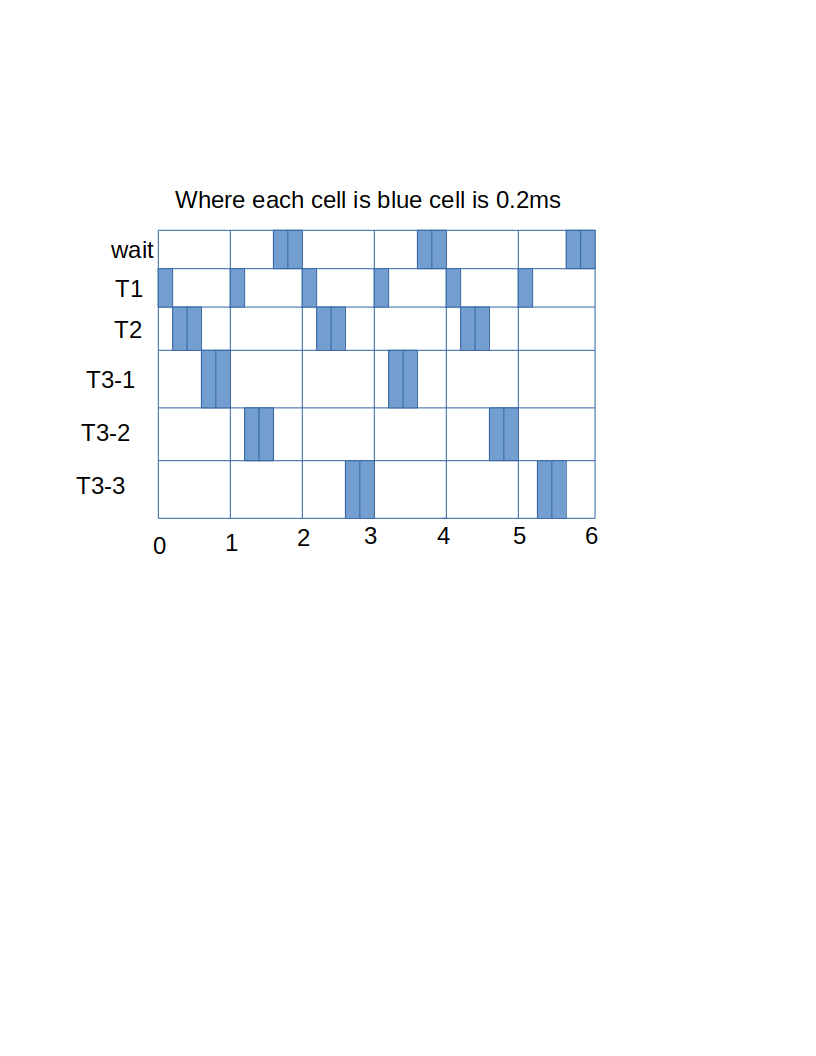
\includegraphics[scale=0.50]{HW2-2.png}
\item Worst case latency is 0.4ms
\end{enumerate}


\end{document}